% !TEX root = ../../../main.tex

\toggletrue{image}
\toggletrue{imagehover}
\chapterimage{dependency}
\chapterimagetitle{\uppercase{Dependency}}
\chapterimageurl{https://xkcd.com/2347/}
\chapterimagehover{Someday ImageMagick will finally break for good and we'll have a long period of scrambling as we try to reassemble civilization from the rubble.}

\chapter{Import und Funktionsaufruf}
\label{chapter-import-funktionsaufruf}

Bisher haben wir beim Programmieren stets von Befehlen gesprochen. Wir haben Befehle verwendet, um die Turtle zu bewegen und zu drehen. In diesem Abschnitt geht es darum, etwas genauer hinzuschauen.
Wir können Befehle in unterschiedliche Kategorie einteilen. Wir befassen uns nun mit den ersten Kategorien, analysieren die bisherigen Befehle und führen neue Fachbegriffe ein. Folgende Ziele erreichen Sie nach diesem Kapitel:

\newcommand{\importFunktionsaufrufLernziele}{
\protect\begin{todolist}
\item Sie erklären die neuen Fachbegriffe und nennen dazu Beispiele.
\item Sie verknüpfen die Fachbegriffe mit einem gegebenen Python-Programm.
\end{todolist}
}

\lernziel{\autoref{chapter-import-funktionsaufruf}, \nameref{chapter-import-funktionsaufruf}}{\protect\importFunktionsaufrufLernziele}

\importFunktionsaufrufLernziele

\section{Befehle analysieren}

Wir besprechen die neuen Fachbegriffe mithilfe von \autoref{lst-quadrat-2}. Es ist das bereits bekannte Programm für ein Quadrat der Seitenlänge $100$. Das Programm besteht aus zehn Befehlen, die wir zwei Kategorien zuordnen können:

\begin{itemize}
	\item \lstinline{import}-Anweisung
	\item Funktionsaufruf
\end{itemize}

Woher weiss ich, zu welcher Kategorie ein Befehl gehört? Dies müssen Sie in der Beschreibung zur Programmiersprache nachlesen. Wir nennen diese Beschreibung, \textbf{Dokumentation}. Die Dokumentation von Python ist unter \url{https://docs.python.org/} abrufbar. Wir fassen in diesen Unterlagen für ausgewählte Befehle das wichtigste aus der Dokumentation zusammen.

\begin{lstlisting}[caption={Python-Programm für ein Quadrat.}, label=lst-quadrat-2]
import turtle

turtle.forward(100)
turtle.left(90)
turtle.forward(100)
turtle.left(90)
turtle.forward(100)
turtle.left(90)
turtle.forward(100)
turtle.left(90)
turtle.done()
\end{lstlisting}

\section{\lstinline{import}-Anweisung}

Der Befehl in der ersten Zeile aus \autoref{lst-quadrat-2} (\lstinline{import turtle}) gehört zur Kategorie \say{\textbf{\lstinline{import}-Anweisung}}.

Möchten wir bestehende Programme in unserem eigenen Python-Programm verwenden, dann können wir die entsprechenden Programme hinzufügen. Dadurch erhalten wir Zugriff auf bereits existierende Befehle. Die \lstinline{import}-Anweisung macht genau dies. Die bestehenden Programme werden \textbf{Module} genannt. Software-Entwickler können Module erstellen und diese zur Verfügung stellen. Jedes Modul besitzt dabei einen \textbf{Namen}. Diesen Namen geben wir bei der \lstinline{import}-Anweisung an. Damit sucht Python nach dem Modul und fügt die darin enthaltenen Programmierelemente dem Programm hinzu. Die \lstinline{import}-Anweisung lautet allgemein:

\begin{center}
\lstinline{import modulname}	
\end{center}

Wir müssen \lstinline{modulname} dann in unserem Programm durch den gewünschten Modulnamen ersetzen. 

\begin{important}
Achten Sie darauf, dass zwischen \lstinline{import}  und dem Modulnamen zwingend ein Leerzeichen eingefügt werden muss.
\end{important}

Es ist die Aufgabe des Programmierers sicherzustellen, dass der Modulname existiert.

\begin{example}
Unsere bisherigen Programme verwenden das Turtle-Modul. Mit \lstinline{import turtle} erhalten wir die Befehle, um die Turtle zu bewegen. Es gibt noch weitere Module, die wir einsetzen werden. Wir können etwa mit \lstinline{import random} Befehle verwenden, um zufällige Zahlen zu erzeugen oder mit \lstinline{import math} erhalten wir Zugriff auf Befehle für mathematische Berechnungen (zum Beispiel Quadratwurzel ermitteln).
\end{example}

\subsection{Worin liegt der Vorteil?} Häufig verwendete Programmierelemente müssen nicht selbst erstellt werden. Wir können auf bestehende Module zurückgreifen und reduzieren dadurch den Programmieraufwand.

\section{Funktionsaufruf}

Die Befehle in den Zeilen drei bis zehn und der Befehl in Zeile zwölf aus \autoref{lst-quadrat-2} gehören alle zur Kategorie \say{\textbf{Funktionsaufruf}}. Jeder dieser Befehle stellt einen Funktionsaufruf (eng. function call) dar.
 
Wir können eine existierende Funktion ausführen, in dem wir einen \textbf{Funktionsaufruf} verwenden. Ein Funktionsaufruf führt Code aus, der unter einem Namen zusammengefasst ist. Wir erkennen einen Funktionsaufruf wie folgt:

\begin{center}
\lstinline{funktionsname(argumente)}	
\end{center}

Ein Argument ist unter anderem eine Zahl oder ein Text, den wir beim Funktionsaufruf übergeben. Es gibt auch Funktionen, die kein Argument oder mehrere Argumente verlangen.

Vorerst \say{bedienen} wir uns an bereits existierenden Funktionen. Wir werden später sehen, wie wir \textbf{selbst} Funktionen erstellen können (Funktionsdefinition).

\begin{figure}[htb]
\centering
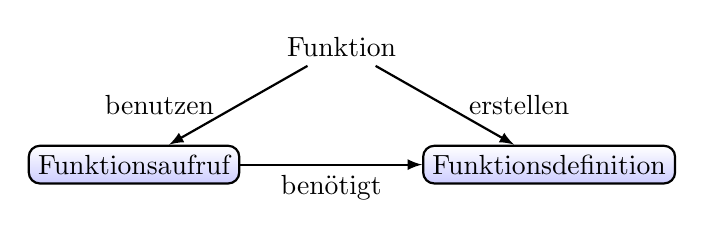
\begin{tikzpicture}[sibling distance=15em, edge from parent/.style = {draw, -latex, thick}]
  \node {Funktion}
    child {	 node[{shape=rectangle, thick, rounded corners,
    draw, align=center, top color=white, bottom color=blue!20}] (call) {Funktionsaufruf} edge from parent node [left, xshift=-0.5em] {benutzen}}
    child { node[{shape=rectangle, thick, rounded corners,
    draw, align=center, top color=white, bottom color=blue!20}] (def) {Funktionsdefinition} edge from parent node [right, xshift=0.5em] {erstellen}};
  \path[-latex, draw, thick] (call) edge node[below] {benötigt} (def);
\end{tikzpicture}
\end{figure}

Schauen wir uns nun einen bekannten Funktionsaufruf im Detail an.

\begin{example}
\label{example-function-call}

Wir rufen die Funktion \lstinline{forward} mit dem Argument \lstinline{100} auf. Da die Funktion aus dem Turtle-Modul stammt, müssen wir den Modulnamen vor den Funktionsaufruf notieren. Modulname und Funktionsaufruf werden durch einen \textbf{Punkt} miteinander verbunden.

$$
\begin{array}[t]{ccc} 
\underbrace{\textrm{\texttt{turtle}}}_{\textrm{Modulname}} & \underbrace{\textrm{\texttt{.}}}_{\textrm{Punkt}} & 
\begin{array}[t]{cccc} 
\underbrace{\textrm{\texttt{forward}}}_{\textrm{Funktionsname}} & \underbrace{\textrm{\texttt{(}}}_{\textrm{öffnende Klammer}} &\underbrace{\textrm{\texttt{100}}}_{\textrm{Argument (eine Zahl)}} & \underbrace{\textrm{\texttt{)}}}_{\textrm{schliessende Klammer}} \end{array} \\
 &  & \underbrace{\hspace{11cm}}_{\textrm{Funktionsaufruf}}
\end{array}
$$

\end{example}

\section{Aufgaben}

In den folgenden Aufgaben repetieren Sie die Fachbegriffe und setzen sich mit der Python-Dokumentation auseinander.

\subsection{Aufgabe 1}

Analysieren Sie alle bisherigen Funktionsaufrufe. Beispiel:

$$
\begin{array}[t]{ccc} 
\underbrace{\textrm{\texttt{turtle}}}_{\textrm{Modulname}} & \texttt{.} & 
\begin{array}[t]{cccc} 
\underbrace{\textrm{\texttt{forward}}}_{\textrm{Funktionsname}} & \texttt{(} &\underbrace{\textrm{\texttt{100}}}_{\textrm{Argument (eine Zahl)}} & \texttt{)} \end{array} \\
 &  & \underbrace{\hspace{6cm}}_{\textrm{Funktionsaufruf}}
\end{array}
$$
\vspace{0.5cm}
\begin{itemize}
	\centering
	\item[] \lstinline{turtle.backward(50)}
	\vspace{1.75cm}
	\item[] \lstinline{turtle.left(90)}
	\vspace{1.75cm}
	\item[] \lstinline{turtle.right(45)}
	\vspace{1.75cm}
	\item[] \lstinline{turtle.pu()}
	\vspace{1.75cm}
	\item[] \lstinline{turtle.pd()}
	\vspace{1.75cm}
	\item[] \lstinline{turtle.done()}
	\vspace{1.75cm}
\end{itemize}

\subsection{Aufgabe 2}

\begin{enumerate}
	\item Wer hat die Idee mit den Turtle-Grafiken erfunden und wann? Sie finden die Antwort in der Dokumentation für das Turtle-Modul. Starten Sie unter \url{https://docs.python.org/3/} und suchen Sie die Webseite des Turtle-Moduls.
	\fillwithlines{0.5in}
	\item Welche Funktionsnamen können Sie für \lstinline{forward}, \lstinline{backward}, \lstinline{left}, \lstinline{right}, \lstinline{penup} und \lstinline{pendown} auch verwenden? Benutzen Sie die Dokumentation.
	\fillwithlines{0.5in}
	\item Mit welchem Funktionsaufruf können Sie die Turtle \say{unsichtbar} machen? Welcher Vorteil ergibt sich dadurch? Wie können Sie die Turtle wieder anzeigen?
	\fillwithlines{1in}
	\item Mit welchem Funktionsaufruf können Sie die Zeichengeschwindigkeit der Turtle beeinflussen? Welche Stufen gibt es?
	\fillwithlines{1in}
\end{enumerate}

\subsection{Aufgabe 3}

Erstellen Sie handschriftlich ein Python-Programm, welches ein Quadrat zeichnet. Die Turtle soll nach der Hälfte des Quadrats unsichtbar werden. Stellen Sie die Zeichengeschwindigkeit der Turtle auf das Minimum (möglichst langsam zeichnen).

\fillwithgrid{\stretch{1}}

\newpage

\subsection{Aufgabe 4}

\begin{enumerate}
	\item Wie berechnen wir mit Python die Quadratwurzel von $42$? Finden Sie die passende Funktion in der Dokumentation des Moduls \lstinline{math}. Notieren Sie den Code hier.
	\fillwithgrid{1.5in}
	\item Wie erzeugen wir mit Python eine Zufallszahl zwischen $1$ und $100$? Finden Sie die passende Funktion in der Dokumentation des Moduls \lstinline{random}. Notieren Sie den Code hier.
	\fillwithgrid{1.5in}
		\item Wie prüfen wir mit Python, ob ein Jahr (z.B. 2017) ein Schaltjahr war? Finden Sie die passende Funktion in der Dokumentation des Moduls \lstinline{calendar}. Notieren Sie den Code hier.
	\fillwithgrid{1.5in}
\end{enumerate}
